\documentclass[18pt]{beamer}
\usepackage[utf8]{inputenc}
\usepackage{templates/mytemplate}
\usepackage{templates/beamerthemekit}
\usepackage{graphicx}
\usepackage{microtype}
\usepackage{listings}
\usepackage{xcolor}
\usepackage{hyperref}
\usepackage{multicol}
\usepackage{siunitx}
\usepackage{physics}

\title{Insights into Tracking in the Belle II Drift Chamber from Cosmic Ray Data}
\subtitle{SUBTITLE}
\author{Michael Eliachevitch}
\date{March 18, 2018}
\titleimage{transparent}
\institute{ETP - KIT}

\begin{document}

  \selectlanguage{english}
  
  \begin{frame}
  \titlepage
\end{frame}

\begin{frame}
  \frametitle{Tracking at Belle II}
  % TODO: image of event display
  \includegraphics[width=.5\textwidth]{figures/Y4S_tagsig.pdf}
  \begin{itemize}
  \item $\sim 11$ tracks from $B$-meson decays
  \item challenges
    \begin{itemize}
    \item full event interpretation: require that all tracks are found\\
      $\rightarrow$ high finding efficiency and low fake rate needed
    \item also for low-$p_T$ tracks
    \item in a high beam background environment
    \end{itemize}
  \item two tracking detectors:
    \begin{itemize}
    \item Vertexdetector System (VXD)
    \item Central Drift Chamber (CDC)
    \end{itemize}
  \end{itemize}
  % B meson decays -> ~11 tracks
  % tracking requirements: 
  % 2 detector systems: VXD and CDC
  % image of the belle 2 tracking detectors
\end{frame}

    
\begin{frame}
  \frametitle{Belle II Drift Chamber}
  
\end{frame}

\begin{frame}
  \frametitle{Cosmics at Belle II}
  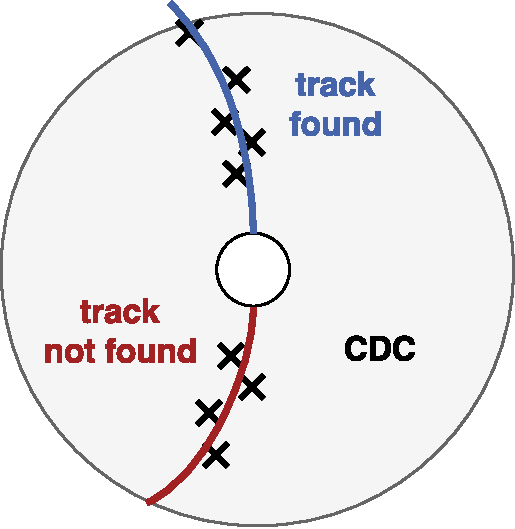
\includegraphics[width=0.5\textwidth]{figures/cdc_finding_fail_diagram.pdf}
\end{frame}




\backupbegin

\begin{frame}
  % \frametitle{Backup-Folien}
  \centering \huge
  Backup
\end{frame}

\begin{frame}
  \frametitle{Track Parameter Distributions}
  
\end{frame}




\end{document}

%%% Local Variables:
%%% coding: utf-8
%%% mode: latex
%%% TeX-engine: default
%%% TeX-master: t
%%% End: